%ASTRONAUT / PORTALS
%
%LAUNCH / PULSAR
%
%VORTEX / ORBIT
%
%GALAXY / BLACKHOLE
%
\begin{center}
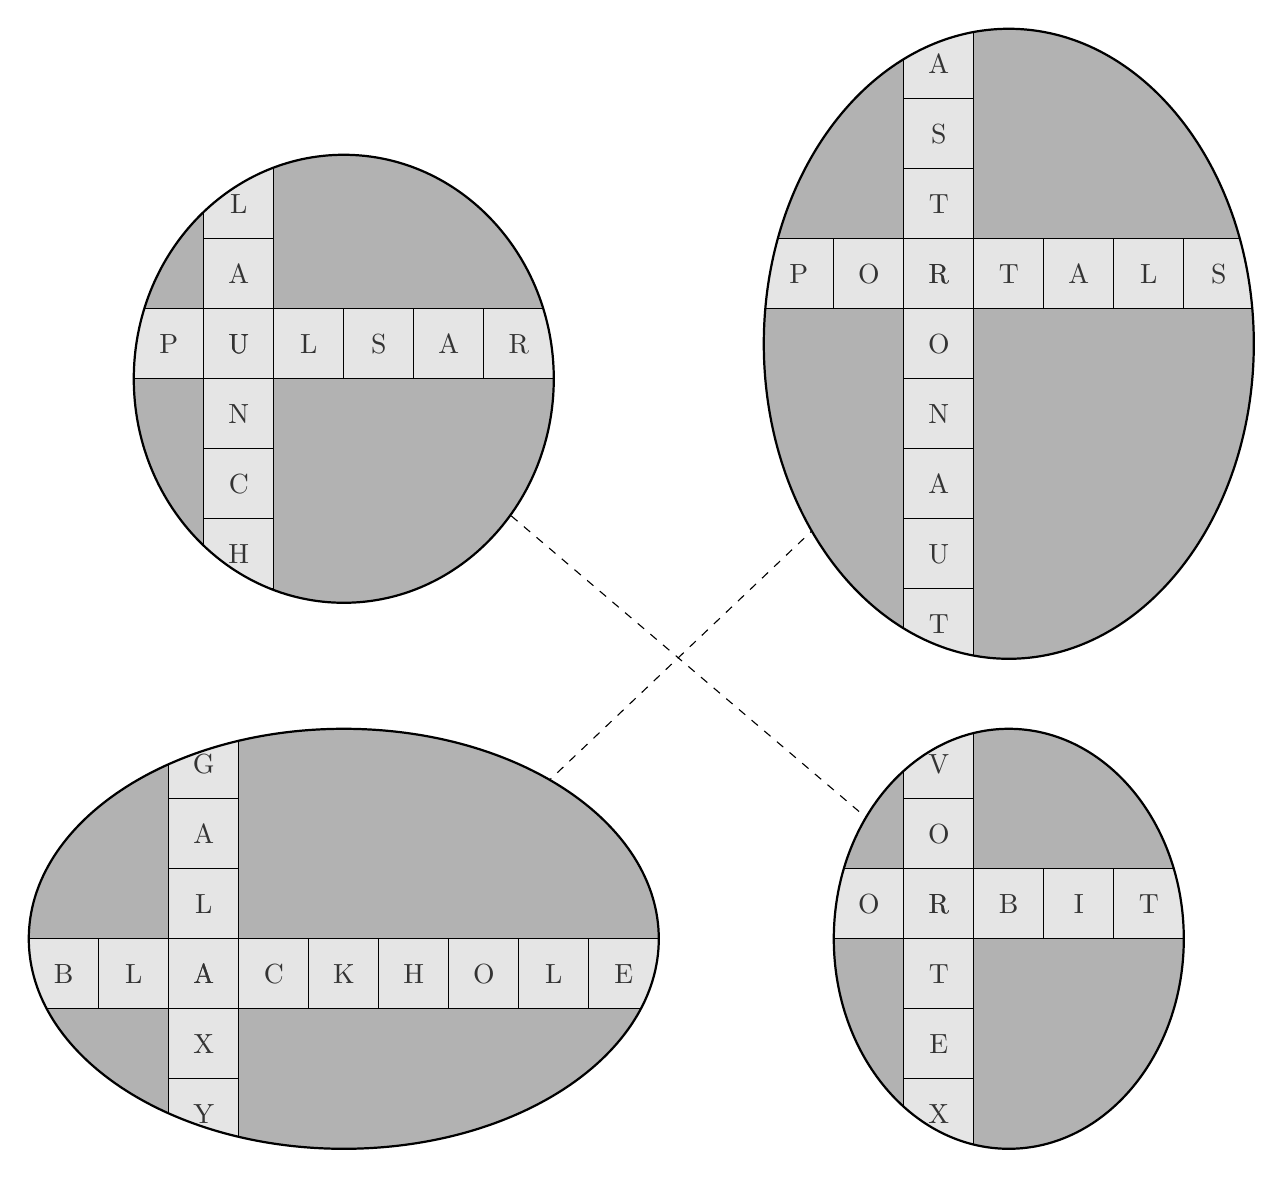
\begin{tikzpicture}[x=0.35in,y=0.35in]
\draw[dashed] (11.5,4.5) -- (1.5,-5);
\draw[dashed] (1.5,4.5) -- (11.5,-4);
\begin{scope}[shift={(10,0)}]
\begin{scope}
\clip (1.5,4.5) ellipse (3.5 and 4.5);
\fill[black!30] (-2,0) rectangle (5,9);
\fill[black!10] (0,0) rectangle (1,9);
\fill[black!10] (-2,5) rectangle (5,6);
\draw[step=1] (0,0) grid (1,9);
\draw[step=1] (-2,5) grid (5,6);
\node[black!80] at (0.5,8.5) {A};
\node[black!80] at (0.5,7.5) {S};
\node[black!80] at (0.5,6.5) {T};
\node[black!80] at (0.5,5.5) {R};
\node[black!80] at (0.5,4.5) {O};
\node[black!80] at (0.5,3.5) {N};
\node[black!80] at (0.5,2.5) {A};
\node[black!80] at (0.5,1.5) {U};
\node[black!80] at (0.5,0.5) {T};
\node[black!80] at (-1.5,5.5) {P};
\node[black!80] at (-0.5,5.5) {O};
\node[black!80] at (0.5,5.5) {R};
\node[black!80] at (1.5,5.5) {T};
\node[black!80] at (2.5,5.5) {A};
\node[black!80] at (3.5,5.5) {L};
\node[black!80] at (4.5,5.5) {S};
%SPROUT
%\node[black!50] at (4.5,5.5) {1};
%\node[black!50] at (-1.5,5.5) {2};
%\node[black!50] at (0.5,5.5) {3};
%\node[black!50] at (0.5,4.5) {4};
%\node[black!50] at (0.5,1.5) {5};
%\node[black!50] at (0.5,6.5) {6};
\end{scope}
\draw[thick] (1.5,4.5) ellipse (3.5 and 4.5);
\end{scope}
\begin{scope}[shift={(0,1)}]
\begin{scope}
\clip (2,3) ellipse (3 and 3.2);
\fill[black!30] (-1,-0.2) rectangle (5,6.2);
\fill[black!10] (0,0) rectangle (1,6);
\fill[black!10] (-1,3) rectangle (5,4);
\draw[step=1] (0,0) grid (1,6);
\draw[step=1] (-1,3) grid (5,4);
\node[black!80] at (0.5,5.5) {L};
\node[black!80] at (0.5,4.5) {A};
\node[black!80] at (0.5,3.5) {U};
\node[black!80] at (0.5,2.5) {N};
\node[black!80] at (0.5,1.5) {C};
\node[black!80] at (0.5,0.5) {H};
\node[black!80] at (-0.5,3.5) {P};
\node[black!80] at (0.5,3.5) {U};
\node[black!80] at (1.5,3.5) {L};
\node[black!80] at (2.5,3.5) {S};
\node[black!80] at (3.5,3.5) {A};
\node[black!80] at (4.5,3.5) {R};
%CAPSULAR
%\node[black!50] at (0.5,1.5) {1};
%\node[black!50] at (3.5,3.5) {2};
%\node[black!50] at (-0.5,3.5) {3};
%\node[black!50] at (2.5,3.5) {4};
%\node[black!50] at (0.5,3.5) {5};
%\node[black!50] at (0.5,5.5) {6};
%\node[black!50] at (0.5,4.5) {7};
%\node[black!50] at (4.5,3.5) {8};
\end{scope}
\draw[thick] (2,3) ellipse (3 and 3.2);
\end{scope}
\begin{scope}[shift={(10,-7)}]
\begin{scope}
\clip (1.5,3) ellipse (2.5 and 3);
\fill[black!30] (-1,-0.2) rectangle (5,6.2);
\fill[black!10] (0,0) rectangle (1,6);
\fill[black!10] (-1,3) rectangle (4,4);
\draw[step=1] (0,0) grid (1,6);
\draw[step=1] (-1,3) grid (5,4);
\node[black!80] at (0.5,5.5) {V};
\node[black!80] at (0.5,4.5) {O};
\node[black!80] at (0.5,3.5) {R};
\node[black!80] at (0.5,2.5) {T};
\node[black!80] at (0.5,1.5) {E};
\node[black!80] at (0.5,0.5) {X};
\node[black!80] at (-0.5,3.5) {O};
\node[black!80] at (0.5,3.5) {R};
\node[black!80] at (1.5,3.5) {B};
\node[black!80] at (2.5,3.5) {I};
\node[black!80] at (3.5,3.5) {T};
%REBOOT
%\node[black!50] at (0.5,3.5) {1};
%\node[black!50] at (0.5,1.5) {2};
%\node[black!50] at (1.5,3.5) {3};
%\node[black!50] at (-0.5,3.5) {4};
%\node[black!50] at (0.5,4.5) {5};
%\node[black!50] at (3.5,3.5) {6};
\end{scope}
\draw[thick] (1.5,3) ellipse (2.5 and 3);
\end{scope}
\begin{scope}[shift={(-0.5,-7)}]
\begin{scope}
\clip (2.5,3) ellipse (4.5 and 3);
\fill[black!30] (-2,0) rectangle (7,6);
\fill[black!10] (0,0) rectangle (1,6);
\fill[black!10] (-2,2) rectangle (7,3);
\draw[step=1] (0,0) grid (1,6);
\draw[step=1] (-2,2) grid (7,3);
\node[black!80] at (0.5,5.5) {G};
\node[black!80] at (0.5,4.5) {A};
\node[black!80] at (0.5,3.5) {L};
\node[black!80] at (0.5,2.5) {A};
\node[black!80] at (0.5,1.5) {X};
\node[black!80] at (0.5,0.5) {Y};
\node[black!80] at (-1.5,2.5) {B};
\node[black!80] at (-0.5,2.5) {L};
\node[black!80] at (0.5,2.5) {A};
\node[black!80] at (1.5,2.5) {C};
\node[black!80] at (2.5,2.5) {K};
\node[black!80] at (3.5,2.5) {H};
\node[black!80] at (4.5,2.5) {O};
\node[black!80] at (5.5,2.5) {L};
\node[black!80] at (6.5,2.5) {E};
%COAXAL
%\node[black!50] at (1.5,2.5) {1};
%\node[black!50] at (4.5,2.5) {2};
%\node[black!50] at (0.5,4.5) {3};
%\node[black!50] at (0.5,1.5) {4};
%\node[black!50] at (0.5,2.5) {5};
%\node[black!50] at (5.5,2.5) {6};
\end{scope}
\draw[thick] (2.5,3) ellipse (4.5 and 3);
\end{scope}
\end{tikzpicture}
\end{center}

The numbered squares spell out the clues
SPROUT, CAPSULAR, REBOOT, and COAXAL.
Drawing lines between these planets on
the Galaxy Map as done
with the insignias targets a fifth planet,
Blurg's home base.
